\chapter{List Views}
\label{LV}

\section{Introduction}
\label{LV:introduction}
\texttt{ListView} is actually a \textit{view group} that contains a list of scrollable items. (Roughly you can think of a list view as a vertical linear layout combined with a scroll bar and a bunch of other functionality!). Just like a vertical linear layout, in a list view you can put simple text view OR very complex layouts inside each row:

\begin{center}
	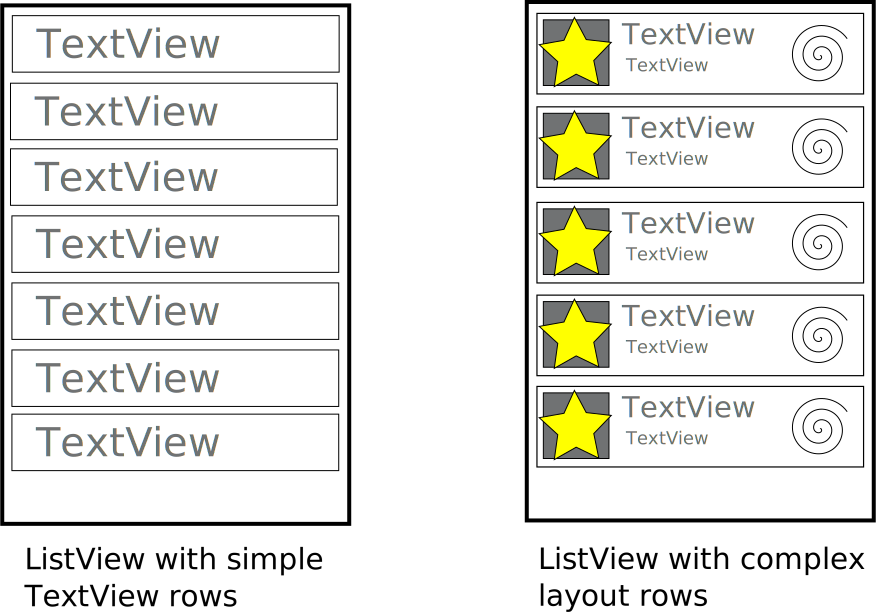
\includegraphics[scale=0.35]{chapters/ch10/images/1}
\end{center}

\begin{quote}
	\textit{``By default each row of the list view contains a single \texttt{TextView} element''.}
\end{quote}

\section{Create New Project}
\label{LV:createProj}

Create a new project from scratch. Perform the following steps:
\begin{enumerate}
	\item Create a new project having name ``\texttt{Chapter\ref{LV}}''
	\item Select minimum API 16 : Android 4.1 (Jelly Bean).
	\item Select ``\texttt{Empty Activity}''
	\item Accept default values for activity and click finish. \\
\end{enumerate}

\section{Populating ListView}
\subsection{Through XML}
Open up to \texttt{activity\_main.xml} and switch to text mode to view its XML code. Change the root layout to \texttt{LinearLayout}. Delete some of its attributes such as padding. Add the orientation attribute and set it to ``vertical'' (line 8). Also remove the default \texttt{TextView} to match the following:

\begin{center}
	\includegraphics[scale=0.4]{chapters/ch10/images/2}
\end{center}

Now change to design mode and drag a ``\textit{list view}'' (from the Containers group) on top of the linear layout. Set list view's width to ``\texttt{match\_parent}'' and it's height to ``\texttt{wrap\_content}'' :

\begin{center}
	\includegraphics[scale=0.4]{chapters/ch10/images/3}
\end{center}

Open ``\texttt{strings.xml}'' and add an ``\texttt{string-array}'' element. This is basically an array of strings. Give it a name such as ``\texttt{employee\_names}'' Each string in this array is specified using an ``\texttt{item}'' tag (lines 4 to 13):

\begin{center}
	\includegraphics[scale=0.4]{chapters/ch10/images/4}
\end{center}

Now open ``\texttt{activity\_main.xml}'' and switch to the text mode. Inside the \texttt{ListView} element add an attribute called ``\texttt{android:entries}'' and assign it a value of ``\texttt{@array/employee\_names}'': (line 14 below):

\begin{center}
	\includegraphics[scale=0.4]{chapters/ch10/images/5}
\end{center}

Switch to the design mode and you will see list view updated with employee names. Also run the app on a device to see the list view in action. Right now clicking on any cell won't do anything but we will soon fix this. \\

The benefit of adding data through XML is that it is easier than other approaches. The drawback, big one, is that the data is fixed and hard coded. Once created you can't grow or shrink the array at runtime.

\subsubsection{Exercise}
Add about 10 more employees to the string array and run the app on a device. Can you scroll the list?

\subsection{Through Java Code}
Before we can proceed, we have to understand the concept of an ``Array Adapter''. 

\subsubsection{The Array Adapter}
The array adapter acts as a glue between the data source and the list view:

\begin{center}
	\includegraphics[scale=0.4]{chapters/ch10/images/6}
\end{center}

For each row in the data source the array adapter creates or ``inflates'' a \texttt{View} for the corresponding row in the list view. In a sense list view is nothing more than an empty shell that is being fed view objects by the array adapter. 

\begin{quote}
	\textit{``By default the array adapter assumes an array of strings as a data source and spits out rows containing a single \texttt{TextView} for the list view. We need to extend the \texttt{ArrayAdapter} class if we want to work with complex data other than strings or if we want to show complex layouts inside list view rows''}.
\end{quote}

Continuing from the previous section open up \texttt{activity\_main.xml} and switch to text mode. Delete the ``\texttt{android:entries}'' tag (line 14 that we added above). Assign an id ``\texttt{employeeList}'' to the list view. The list view element should look like following:

\begin{center}
	\includegraphics[scale=0.4]{chapters/ch10/images/7}
\end{center}

Open up \texttt{MainActivity.java} and in \texttt{onCreate} function, add an array of strings which will act as the data source. Also obtain the reference to our \texttt{ListView} that we added initially (lines 14-21):

\begin{center}
	\includegraphics[scale=0.4]{chapters/ch10/images/8}
\end{center}

Final step is to create an \texttt{ArrayAdapter} object and attach it to the list view. Add the following code right after line 21:

\begin{center}
	\includegraphics[scale=0.4]{chapters/ch10/images/9}
\end{center}

Let's review the code line by line:

\begin{itemize}
	\item \textit{Line 22:} The array adapter constructor that we're using accepts three arguments. First one is the current context which will be '\texttt{this}' in most cases.
	
	\item \textit{Line 23:} Here you specify the layout that will be used to create each list view row. We are using a default layout provided by android named \texttt{simple\_list\_item\_1}. This is why we added the \texttt{android} keyword before the name because it belongs to the android namespace.
	
	\item \textit{Line 24:} Specify the data source, which in this case, is an array of strings that we created earlier.
	
	\item \textit{Line 25:}  Finally attach the array adapter object to the list view.
\end{itemize}

Run this app and you will see a bunch of entries in the list view. As usual you can click these but nothing will happen yet. \\

Let's explore \texttt{simple\_list\_item\_1} a bit more. Go to line 23 and right click on the \texttt{simple\_list\_item\_1} name, a popup menu will appear. Select ``Go to $\rightarrow$ Declaration'', an xml file named \texttt{simple\_list\_item\_1.xml} will open up in the designer window. If you look at it closely you'll notice that this layout file contains only one \texttt{TextView} widget, exactly as we claimed earlier:

\begin{center}
	\includegraphics[scale=0.4]{chapters/ch10/images/10}
\end{center}

You can also switch to text mode and take a look at its xml source code.

\subsection{Providing Complex Data Source}
Right click on the package name group and create a new class called ``\texttt{Employee}'':

\begin{center}
	\includegraphics[scale=0.4]{chapters/ch10/images/11}
\end{center}

Open up \texttt{Employee} class and add member variables as follows (note they are all private):

\begin{center}
	\includegraphics[scale=0.4]{chapters/ch10/images/12}
\end{center}

Left-click anywhere inside the class. Then right click and select ``\texttt{Generate}'', then from the popup menu select ``\texttt{Constructor}''. From the window select all the variables at once using shift key and hit generate:

\begin{center}
	\includegraphics[scale=0.4]{chapters/ch10/images/13}
\end{center}

A constructor will be created in the class. You can also write it manually:

\begin{center}
	\includegraphics[scale=0.4]{chapters/ch10/images/14}
\end{center}

Open up ``\texttt{MainActivity.java}''. Inside the \texttt{onCreate} method, delete the previous code that we wrote and create a list of \texttt{Employees} and populate with some values (the more entries the better). Also get the reference for our list view object and create an array adapter. Note that the array adapter will now be of type \texttt{Employee} instead of \texttt{String} (lines 14 to 23):

\begin{center}
	\includegraphics[scale=0.4]{chapters/ch10/images/15}
\end{center}

If you run the app on a device it shows the following output:

\begin{center}
	\includegraphics[scale=0.4]{chapters/ch10/images/16}
\end{center}

In java the \href{https://developer.android.com/reference/java/lang/Object.html}{\texttt{Object}} class is the parent class of all classes. Whenever you try to print an object or convert it into a \texttt{String} the \texttt{Object} class's ``\texttt{toString}'' method is called. By default it returns a string containing object specific details such as its reference. Since the default array adapter is expecting a string data source by default, it tries to convert \texttt{Employee} object into a \texttt{String}, and hence the reason you are seeing the above output. We can easily override this method to create a string of our own choice:

\begin{center}
	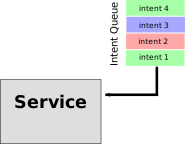
\includegraphics[scale=0.4]{chapters/ch10/images/17}
\end{center}

yielding the following output in desired format:

\begin{center}
	\includegraphics[scale=0.4]{chapters/ch10/images/18}
\end{center}

Or you can also return something a bit more complex:

\begin{center}
	\includegraphics[scale=0.4]{chapters/ch10/images/19}
\end{center}

resulting in the output:

\begin{center}
	\includegraphics[scale=0.4]{chapters/ch10/images/20}
\end{center}

We know that the default input data source for array adapters is \texttt{String}. Also the default view that the array adapter generates against each data row is a single \texttt{TextView}. So let's hack it a little bit and try to change the default outlook by specifying our own simple layout file. \\

Create a new layout named ``\texttt{listview\_simple\_layout.xml}''. Open it up in text mode and delete the root element. Now add a single \texttt{TextView} object inside this file. As opposed to \texttt{activity\_main.xml} (or any activity layout file) there is no root layout here:

\begin{center}
	\includegraphics[scale=0.4]{chapters/ch10/images/21}
\end{center}

You may see the keyword \texttt{android} highlighted in red. The reason for this is that we didn't specify the android namespace in our xml code. Place the keyboard cursor on the \texttt{android} keyword, a tool tip appears asking you to press \texttt{Alt+Enter}:

\begin{center}
	\includegraphics[scale=0.4]{chapters/ch10/images/22}
\end{center}

Pressing \texttt{Alt+Enter} will bring up a popup menu. Select ``Create namespace declaration'':

\begin{center}
	\includegraphics[scale=0.4]{chapters/ch10/images/23}
\end{center}

This will automatically add the necessary definitions and namespaces as shown below (line 6):

\begin{center}
	\includegraphics[scale=0.4]{chapters/ch10/images/24}
\end{center}

Switch to design mode. You should see a simple text view rendered without any issues. Change its properties to match the following:

\begin{center}
	\includegraphics[scale=0.4]{chapters/ch10/images/25}
\end{center}

Go back to \texttt{MainActivity.java} and replace ``android.R.layout.simple\_list\_item\_1'' with our custom layout ``R.layout.listview\_simple\_layout'' that we just created (line 21):

\begin{center}
	\includegraphics[scale=0.4]{chapters/ch10/images/26}
\end{center}

Note that we are NOT appending it with \texttt{android} keyword because our layout does not reside in the default android namespace, it is inside our project namespace. \\

If you run this on a device you will see the changed outlook:

\begin{center}
	\includegraphics[scale=0.4]{chapters/ch10/images/27}
\end{center}

If you click any row nothing seems to work. But don't worry the system is properly registering your clicks. It is just that it has disabled its animations because you specified your own custom background. If you set the background to nothing and run the app again, you will notice the animations coming back when you click any entry.

\subsection{Exercise}
\begin{enumerate}
	\item Add more data (i.e Employees) so that the list becomes scrollable.
	\item Try changing the outlook of the rows to something interesting.
\end{enumerate}

\section{Handling Input Events}
As we did with the buttons registering click events is pretty simple and straightforward. But instead of using \texttt{onClick} event, we will now set the \texttt{onItemClick} listener. Add the following code right after our previous code (lines 28 to 33 below):

\begin{center}
	\includegraphics[scale=0.4]{chapters/ch10/images/28}
\end{center}

Notice line 30 above, the event handler method. We are interested in the \texttt{position} parameter. This parameter tells us the index of the corresponding data element on which the user clicked. The \texttt{view} parameter gives us the entire view object for that particular row. This can be as simple as a text view or very complex layouts within layouts. Let's read the string from the row and display it in a toast. Inside the \texttt{onItemClick} listener method add the following code (lines 32 to 36):

\begin{center}
	\includegraphics[scale=0.4]{chapters/ch10/images/29}
\end{center}

We know for sure that by default array adapter generates a single text view for each for of the list view. So in line 38 we are just casting the view into a \texttt{TextView}. Then in line 39 we are reading its string value. Finally in line 40 display the position index of the selected row along with its visible string. Notice that in line 40 ``\texttt{MainActivity.this}'' is being passed instead of just ``\texttt{this} as the current context.


